\documentclass{beamer}
\beamertemplatenavigationsymbolsempty
\usecolortheme{beaver}
\setbeamertemplate{blocks}[rounded=true, shadow=true]
\setbeamertemplate{footline}[page number]
%
\usepackage[utf8]{inputenc}
\usepackage[english]{babel}
\usepackage{amssymb,amsfonts,amsmath,mathtext}
\usepackage{subfig}
\usepackage[all]{xy} % xy package for diagrams
\usepackage{array}
\usepackage{multicol}% many columns in slide
\usepackage{hyperref}% urls
\usepackage{hhline}%tables

\usepackage[backend=biber,style=authoryear]{biblatex}
\bibliography{../article/draft_lib} % assumes refs.bib includes the entry

% Your figures are here:
\graphicspath{ {fig/} {../figs/} }
\newcommand{\eqdef}{\stackrel{\Delta}{=}}
\newcommand{\SG}{\mathrm{SG}}
\newcommand{\rd}[3]{\mathrm{D}_{#1}\infdivx*{#2}{#3}}
\newcommand{\rdalpha}[2]{\mathrm{D}_{\alpha}\infdivx*{#1}{#2}}
\newcommand{\renyi}{R\'enyi}
\newcommand{\erfc}{\mathrm{erfc}}
\newcommand{\eps}{\varepsilon}
\usepackage{mathtools}
\DeclarePairedDelimiterX{\infdivx}[2]{(}{)}{#1\;\delimsize\|\;#2}
%----------------------------------------------------------------------------------------------------------
\title[\hbox to 56mm{Feature generation}]{Differentially private modification of sign-SGD}
\author[A.\,Yu.~Kravatskiy]{Alexey Kravatskiy}
\institute{Moscow Institute of Physics and Technology}
\date{\footnotesize
\par\smallskip\emph{Course:} My first scientific paper\par (Strijov's practice)/Group 205 %821, 813
\par\smallskip\emph{Expert:} A.\,N.~Beznosikov
\par\smallskip\emph{Consultant:} S.\,A.~Chezhegov
\par\bigskip\small 2025}

%----------------------------------------------------------------------------------------------------------
\begin{document}
%----------------------------------------------------------------------------------------------------------
\begin{frame}
\thispagestyle{empty}
\maketitle
\end{frame}
%-----------------------------------------------------------------------------------------------------
\begin{frame}{Distributed, Private, and Noise-resistant}
\begin{block}{Goal}
A communication-efficient and private algorithm for distributed optimization converging under heavy-tailed noise (noise with unbounded variance).
\end{block}
\begin{block}{Problem}
The only proposed private sign-based algorithm dp-signSGD either is not private or does not converge.
\end{block}
\begin{block}{Solution}
A new privacy accountant for dp-signSGD that affords lower noise to ensure privacy.
\end{block}
\end{frame}
%-----------------------------------------------------------------------------------------------------
\begin{frame}{Differential privacy of DP-signSGD}

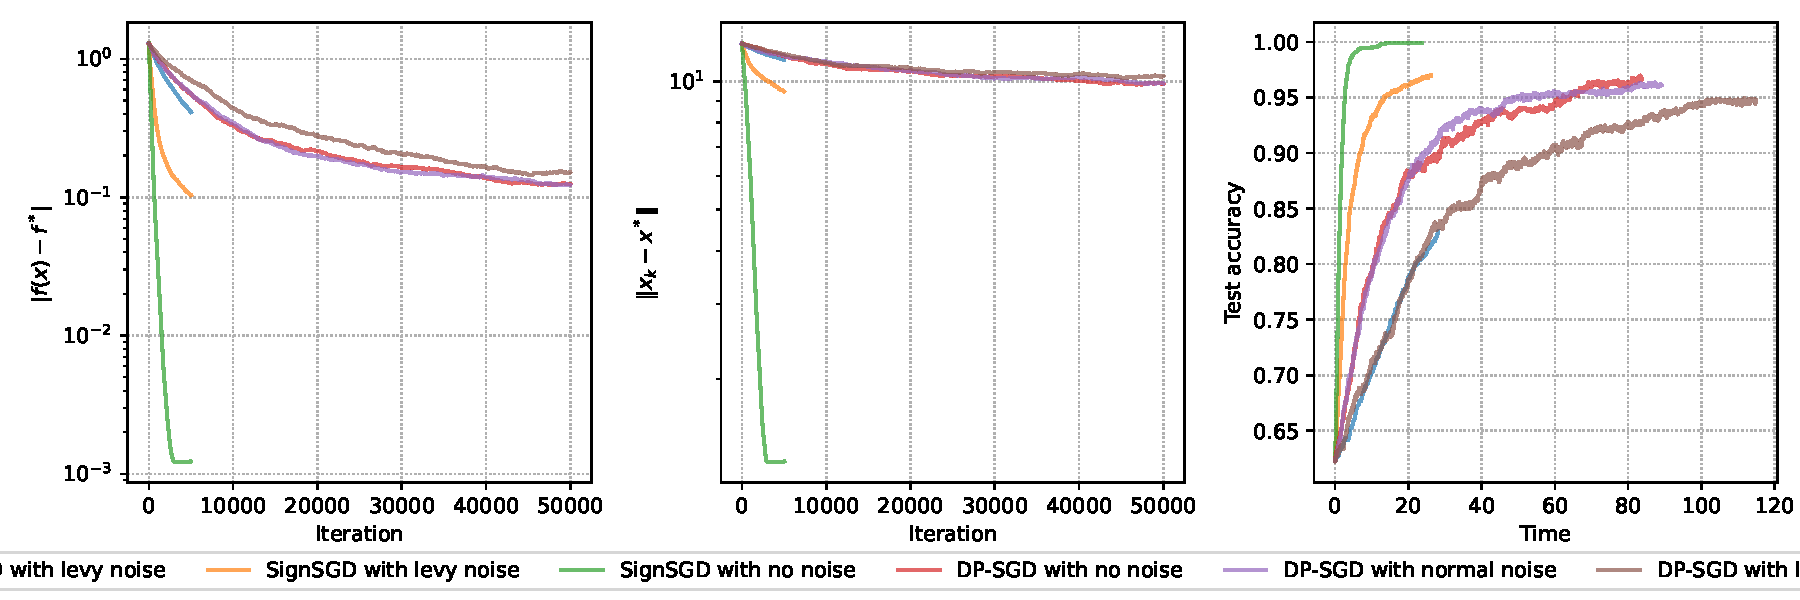
\includegraphics[width=1.0\textwidth]{dp_sign_converges} 

\bigskip
DP-signSGD with an appropriate $\sigma$ is {\color{red} $(\epsilon, delta)$-private and converges under heavy-tailed noise}.
\end{frame}

%-----------------------------------------------------------------------------------------------------
\begin{frame}{Literature}
\nocite{Jin2020}
\nocite{Mironov2017}
\nocite{mironov2019SGM}
\printbibliography
\end{frame}

%----------------------------------------------------------------------------------------------------------
\begin{frame}{Differential Privacy}
    \begin{definition}
        Given a set of local datasets $\mathcal{D}$ provided with a notion of neighboring local datasets $\mathcal{N}_{\mathcal{D}}\subset \mathcal{D}\times \mathcal{D}$ that differ in only one data point. For a query function $f: \mathcal{D}\rightarrow \mathcal{X}$, a mechanism $\mathcal{M}:\mathcal{X}\rightarrow \mathcal{O}$ to release the answer of the query is defined to be $(\epsilon,\delta)$-locally differentially private if for any measurable subset $\mathcal{S}\subseteq\mathcal{O}$ and two neighboring local datasets $(D_1,D_2)\in \mathcal{N}_{\mathcal{D}}$,
        \begin{equation}
        P(\mathcal{M}(f(D_1))\in \mathcal{S}) \leq e^{\epsilon}P(\mathcal{M}(f(D_2))\in \mathcal{S}) + \delta.
        \end{equation}
    \end{definition}
        
        A key quantity in characterizing local differential privacy for many mechanisms is the sensitivity of the query $f$ in a given norm $l_{r}$, which is defined as
        \begin{equation}\label{sensitivity}
        \Delta_{r} = \max_{(D_1,D_2)\in\mathcal{N}_{\mathcal{D}}}||f(D_1)-f(D_2)||_r.
        \end{equation}
\end{frame}
%-----------------------------------------------------------------------------------------------------
\begin{frame}{Rényi divergence (\cite{Mironov2017})}
    \begin{definition}[\renyi\ divergence] Let $P$ and $Q$ be two distributions on $\mathcal{X}$ defined over the same probability space, and let $p$ and $q$ be their respective densities. The \renyi\ divergence of a finite order $\alpha\neq 1$ between $P$ and $Q$ is defined as
        \[
        \rdalpha{P}{Q}\eqdef \frac1{\alpha-1}\ln \int_{\mathcal{X}} q(x)\left(\frac{p(x)}{q(x)}\right)^{\alpha}\,\mathrm{d}x.
        \]
        \renyi\ divergence at orders $\alpha=1,\infty$ are defined by continuity.
        \end{definition}
        
        
    
\end{frame}
%-----------------------------------------------------------------------------------------------------
\begin{frame}{Rényi differential privacy (\cite{Mironov2017})}
    \begin{definition}[\renyi\ differential privacy (RDP)] We say that a randomized mechanism $\mathcal{M}\colon \mathcal{S}\to\mathcal{R}$ satisfies $(\alpha,\eps)$-\renyi\ differential privacy (RDP) if for any two \emph{adjacent} inputs $S,S'\in \mathcal{S}$ it holds that
        \[
        \rdalpha{\mathcal{M}(S)}{\mathcal{M}(S')}\leq \eps.
        \]
        \end{definition}
        
    
\end{frame}
%-----------------------------------------------------------------------------------------------------
\begin{frame}{Sample Gaussian Mechanism (\cite{mironov2019SGM})}
    \begin{definition}[Sampled Gaussian Mechanism (SGM)] Let $f$ be a function mapping subsets of $\mathcal{S}$ to $\mathbb{R}^d$. We define the Sampled Gaussian mechanism (SGM) parameterized with the sampling rate $0<q\leq 1$ and the noise $\sigma>0$ as
        \[
        \SG_{q,\sigma}(S)\eqdef f(\{x\colon x\in S \textrm{ is sampled with probability } q\})+\mathcal{N}(0,\sigma^2\mathbb{I}^d),
        \]
    where each element of $S$ is sampled independently at random with probability $q$ without replacement, and $\mathcal{N}(0,\sigma^2\mathbb{I}^d)$ is spherical $d$-dimensional Gaussian noise with per-coordinate variance $\sigma^2$.
    \end{definition}
    
    \end{frame}
%-----------------------------------------------------------------------------------------------------
\begin{frame}{Criterion of a private algorithm}
Following the procedure from \cite{mironov2019SGM}, we can get:
$$\eps_R \leq \frac{1}{\alpha - 1} \log\left(\sum_{k=0}^{\alpha} {\alpha \choose k}  (1-q)^{\alpha-k}q^{k} \exp\left(\frac{k^2 - k}{2\sigma^2}\right)\right)$$

While according to the advanced composition theorem and conversion from \renyi  privacy to $(\eps, \delta)$-privacy, $\eps_R$ must satisfy:
$$ \eps_R \leq \eps/T - \frac{\log 1/\delta}{T(\alpha - 1)}$$.
\end{frame}

%----------------------------------------------------------------------------------------------------------
\begin{frame}{Grid Search to find minimal $\sigma$}
\begin{columns}[c]
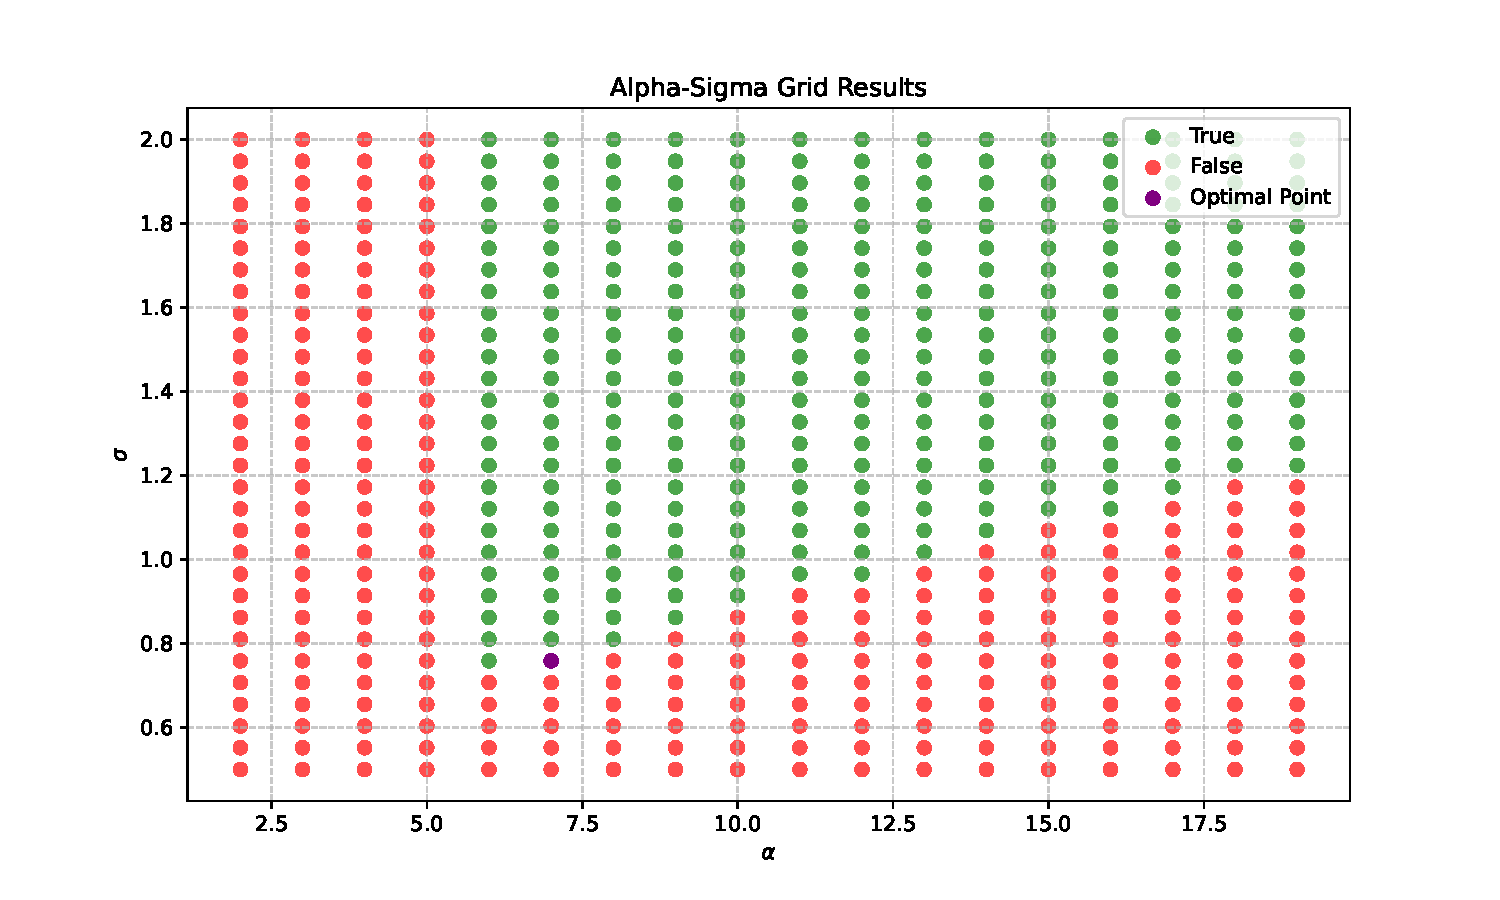
\includegraphics[width=1.0\textwidth]{valid_sigma} 
\end{columns}
\end{frame}
%----------------------------------------------------------------------------------------------------------
\begin{frame}{Computational experiment}
    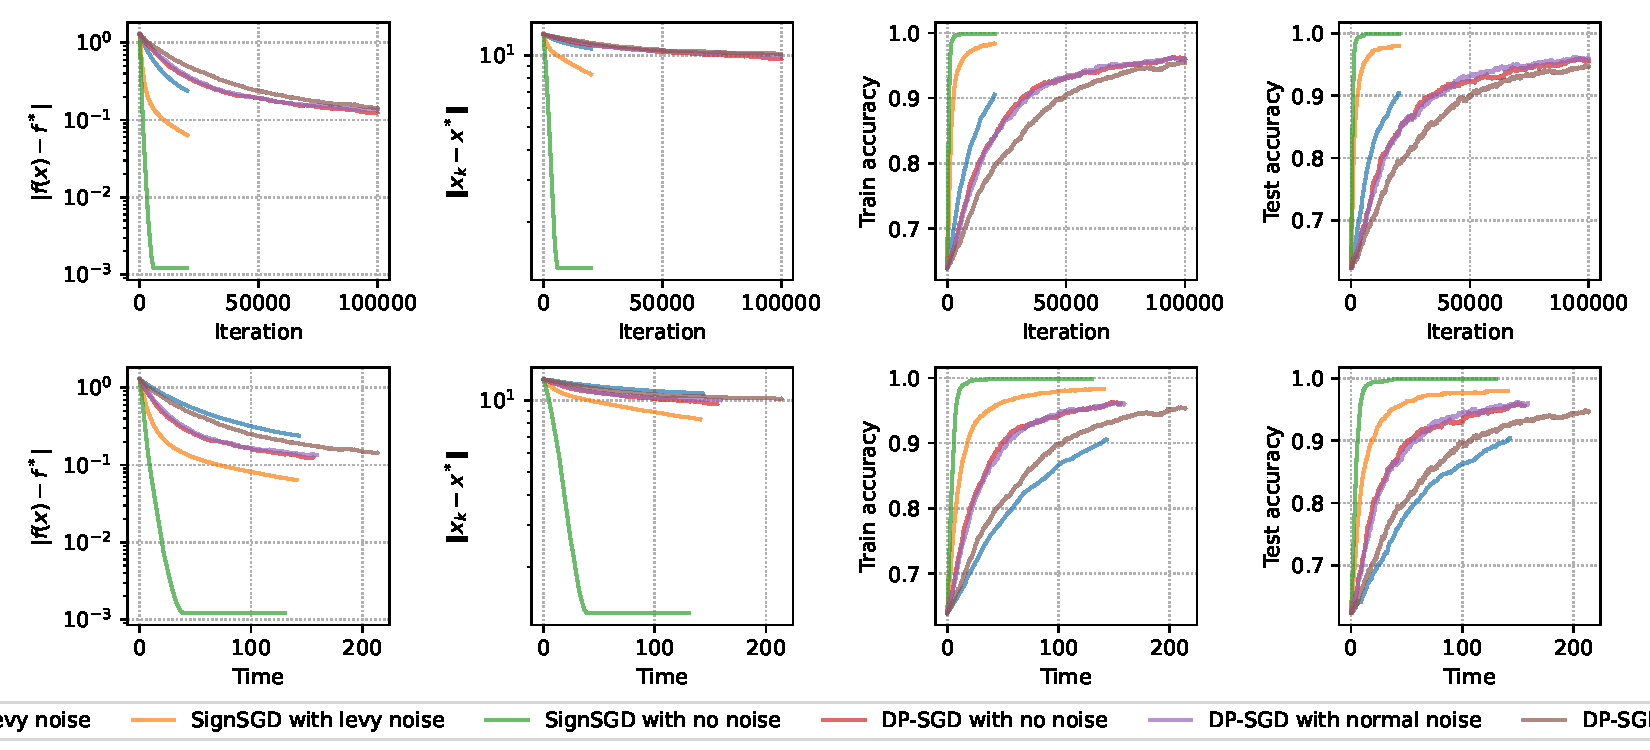
\includegraphics[width=1.0\textwidth]{dp_sign_100K_steps} 
dp-sign SGD converges very slowly, but it depends on a dataset. Lower $q$ leads to much lower $\sigma$ and better convergence.
\end{frame}
%----------------------------------------------------------------------------------------------------------
\begin{frame}{Conclusion}
    \begin{block}{dp-sign SGD}
    \begin{itemize}
        \item with Poisson sampling $q = 1/n$ 
        \item is $(10, 1/n^{1.1})$ differentially-private
        \item empirically converges on logistic regression problem even with heavy-tailed noise
    \end{itemize}
    \end{block}
    Now we have to provide theoretical guarantees of convergence.
\end{frame}
%----------------------------------------------------------------------------------------------------------
\end{document} 